\documentclass{article}
\usepackage{listings}
\usepackage{graphicx} % Required for inserting images
\usepackage{color}
\usepackage[a4paper, total={6.5in, 10in}]{geometry}
\usepackage{enumitem}

\lstnewenvironment{C}
  {\lstset{language=C}} 
%Add your addition parameters as required like showstringspaces , line numbering , 
% frames , etc.seperated by a comma as shown in the CPP  environment 
  {}
\lstnewenvironment{CPP}
  {\lstset{language=C++,basicstyle=\ttfamily\small,frame=none}}
  {}
\lstnewenvironment{Java}
  {\lstset{language=Java}}
  {}
\lstnewenvironment{Python}
  {\lstset{language=Python}}
  {}

% \title{\huge TP3 Report \\ Artificial Intelligence}
% \author{Bruno Luiz Dias Alves de Castro \\ Victor Gabriel Mendes Sündermann}
% \date{April 2023}

\begin{document}

\begin{titlepage}
\centering
{\textsc{\Large ESIEE Paris \\ ~\\ Artificial Intelligence and Cybersecurity} \par}
\vfill
{\huge\bfseries Network Security \par}
\vspace{0.5cm}
{\LARGE Lab 3 Report \par}
\vspace{2cm}
{\Large\itshape Bruno Luiz Dias Alves de Castro \par}
{\Large\itshape Victor Gabriel Mendes Sündermann \par}
\vfill

% Bottom of the page
{\large \today\par}
\end{titlepage}

\pagebreak
\tableofcontents
\pagebreak

\section{Introduction}

This report is constituted of two parts, the first one aims to create and configure a DNS server and to study the attacks that can be done on it.
The attacks tackeld in this part are: DNS cache poisoning, spoofing DNS responses and sniffing and spoofing of packets.
The second part is an implementation of a Firewall to filter packets and block the communication between two machines.

\section{Part1: Local DNS Attack}
\subsection{Setting up the environment}
In order to set up the Virtual Machines we used the Oracle VMBox to set them up and utilized a Debian Linux image, the IP of the machines were set as following:
User: 10.0.2.18
Attacker: 10.0.2.17
Server: 10.0.2.16

After creating and configuring the VM's they were connected to the same NAT network which has the address: 

For the server to be initialized it's necessary to run a DNS server software, for this lab the BIND9 was used and the following figure shows that rhe server was able to communicate with external webites:

\begin{center}
  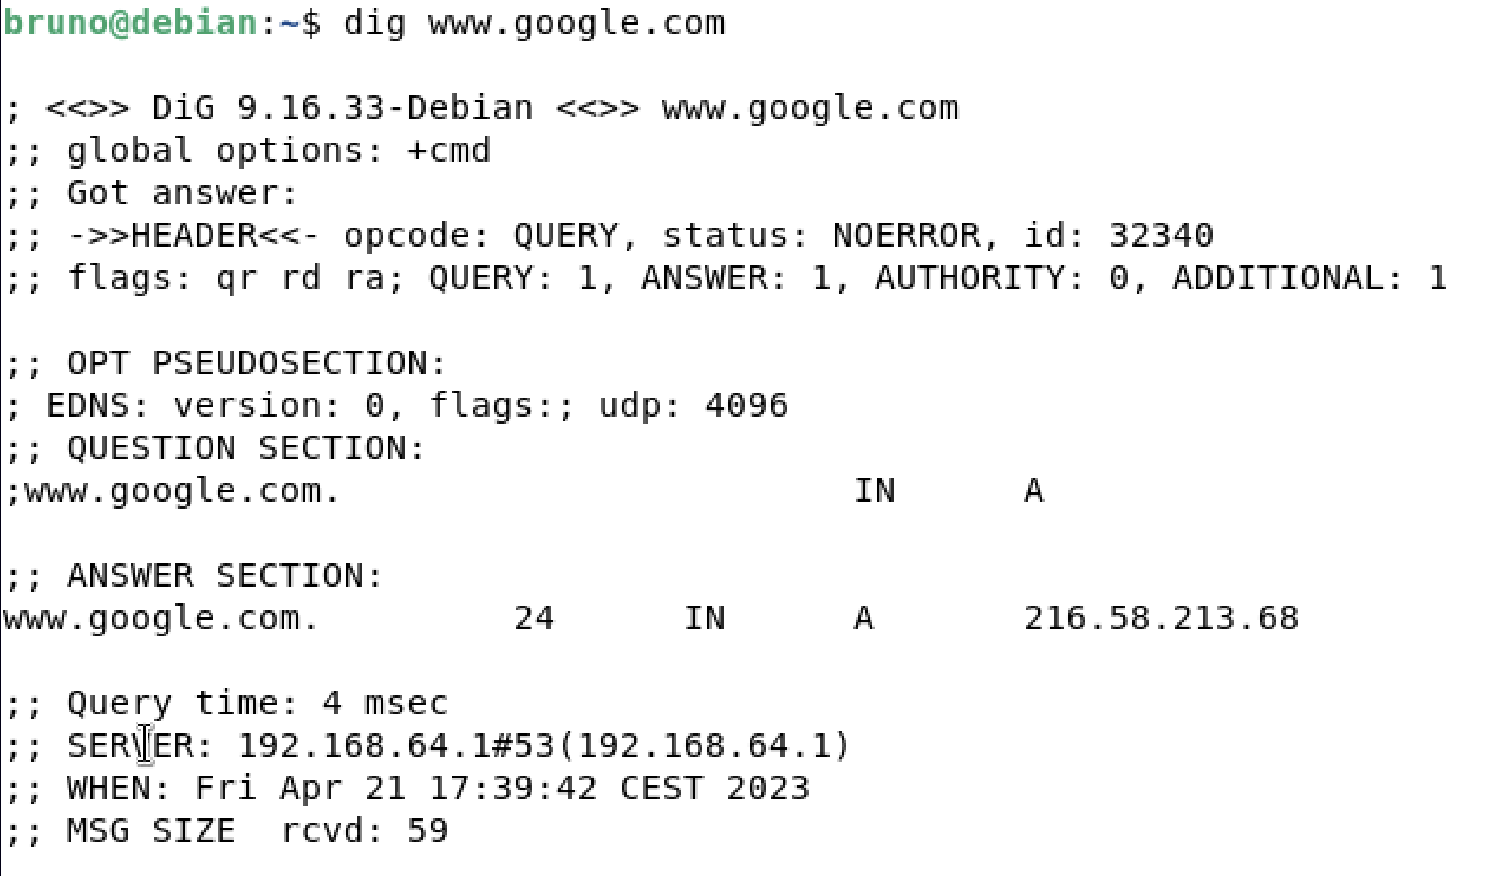
\includegraphics[scale=0.5]{images/dig-google.png}
\end{center}

Now that our server is running we can visualize the packets that went trought it with Wireshark, the picture bellow shows the results from a ping to Google's website:

\begin{center}
  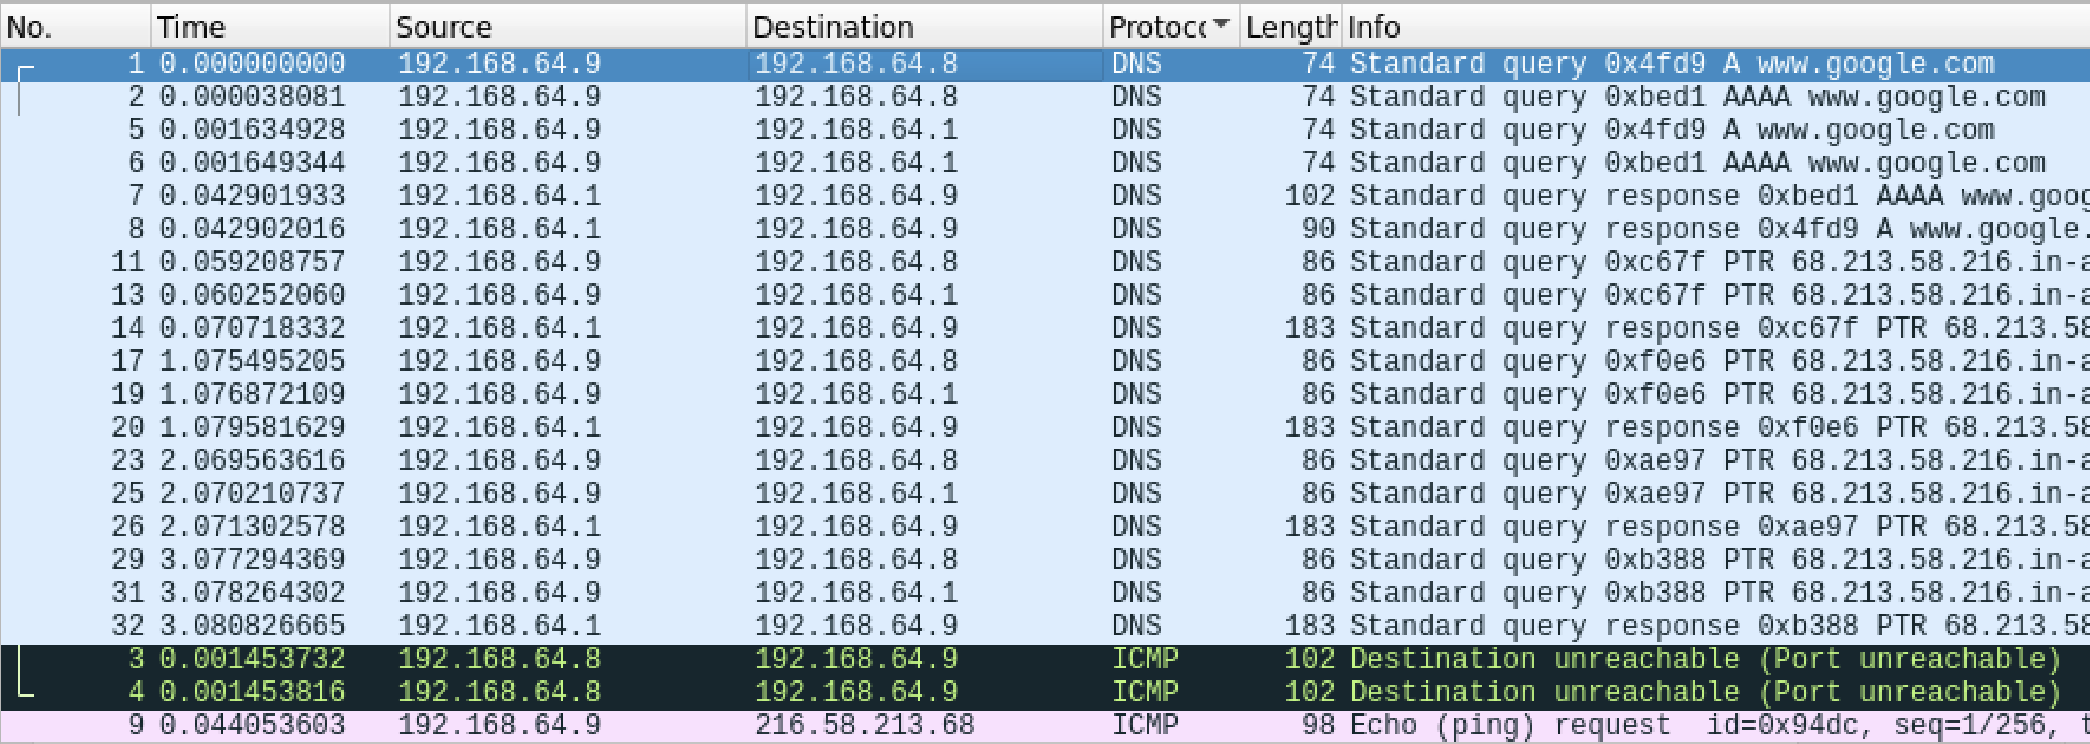
\includegraphics[scale=0.4]{images/ping-google.png}
\end{center}

But a problem arises as the server is unreachable, this is caused by adding the following line of code requested at Step 1 from Task 2, ultimately causing the server to not be initialized.

\hbox{}

\definecolor{light-gray}{gray}{0.95}
\begin{lstlisting}[language=bash, frame=tlbr, framesep=6pt, backgroundcolor=\color{light-gray}]
  options{
    dump-file "/var/cache/bind/dump.db";
  };
\end{lstlisting}

After following the next steps, if the code is run without the line mentioned above we can run it without errors.

At task 3 we configure a zone so that the DNS server is able to retrieve data from other domains, on step 2 the code given was wrong, so the group had to rewrite it in order to make it functional, the resulting code can be seen bellow:

\begin{center}
  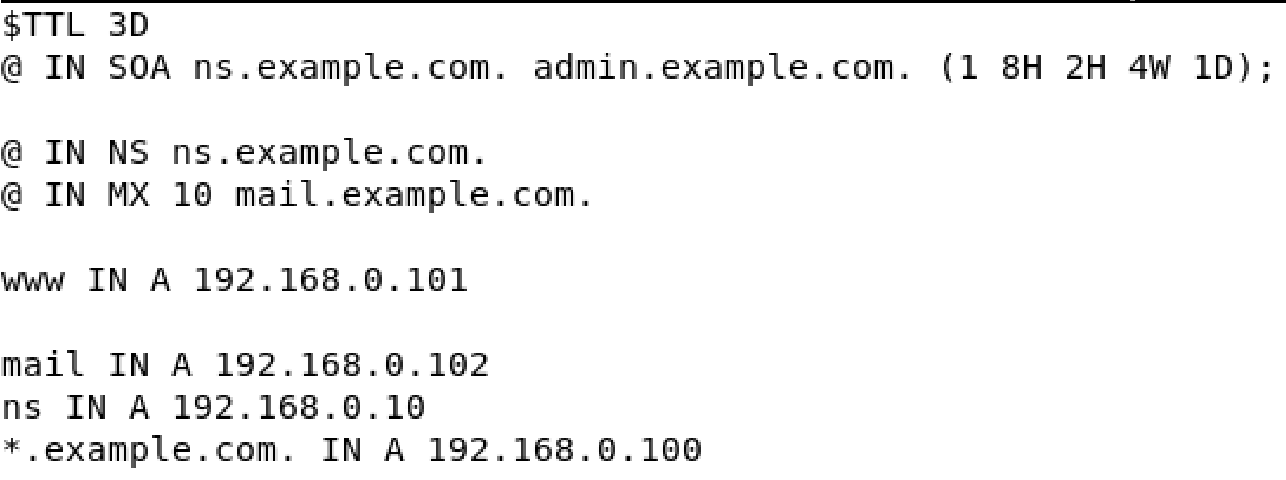
\includegraphics[scale=0.5]{images/bind-config-corrected.png}
\end{center}

After running the corrected code we can see that the server is able to retrieve data from other domains, we then add the line of code that was creating an error before, after this, steps 3 and 4 were run without any changes to the code.
The result can be seen bellow when we run the dig command to retrieve data from the example.com domain:

\begin{center}
  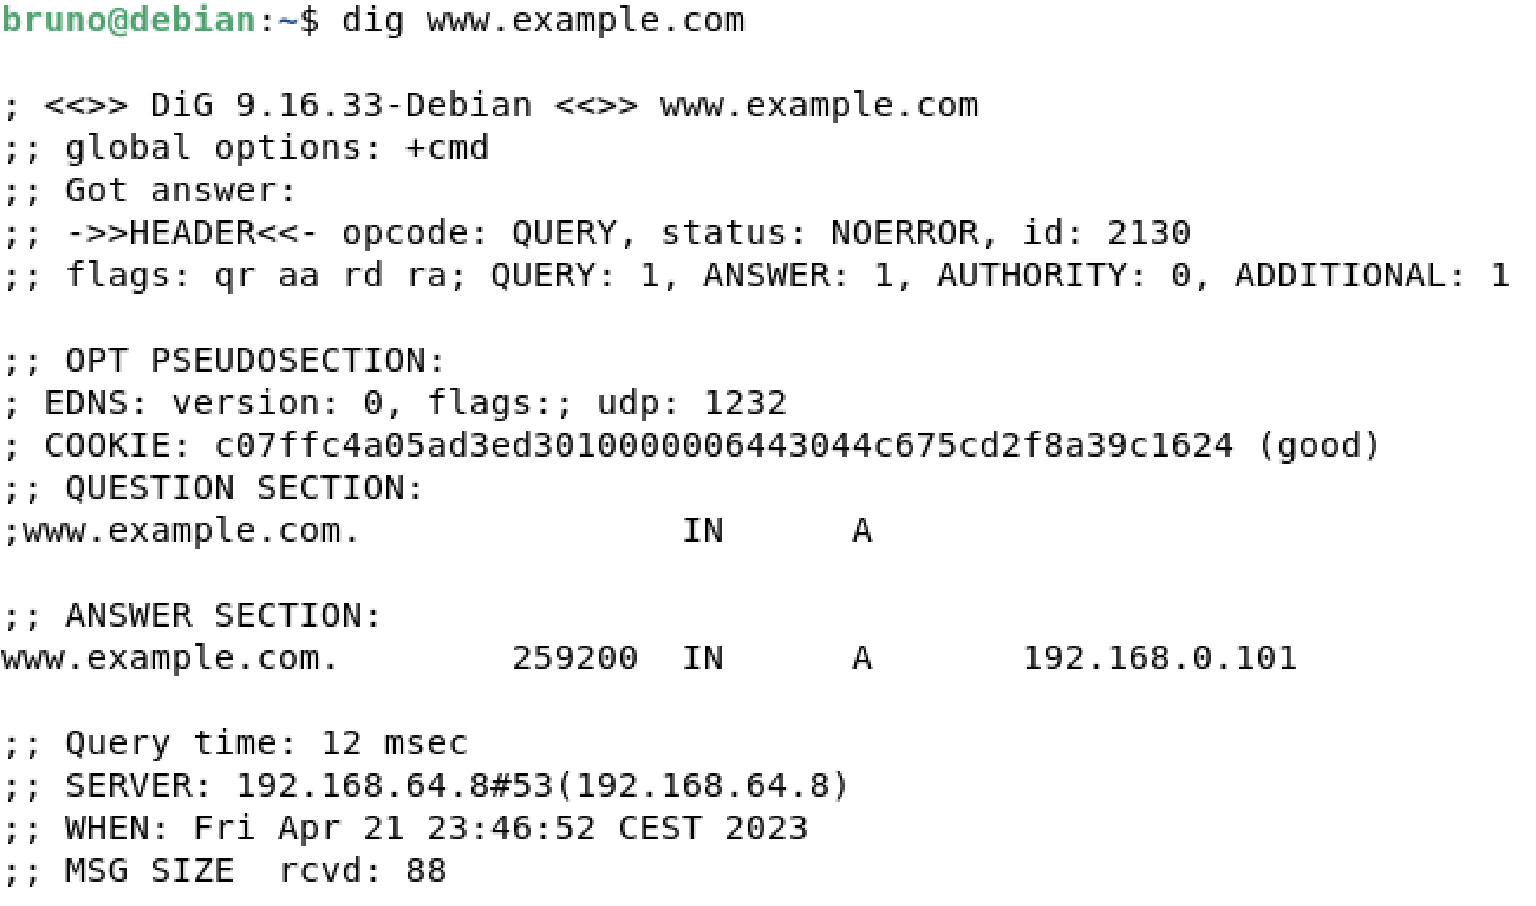
\includegraphics[scale=0.5]{images/dig-examplecom.png}
\end{center}


Now that the server is successfully functioning it's time to realize a Spoofing attack, this is done by running the command 'netwox'and sending the IPs of the server, the targeted website and to wich IP the victim will be redirected.
Bellow is a photo of the command and it's result:

\begin{center}
  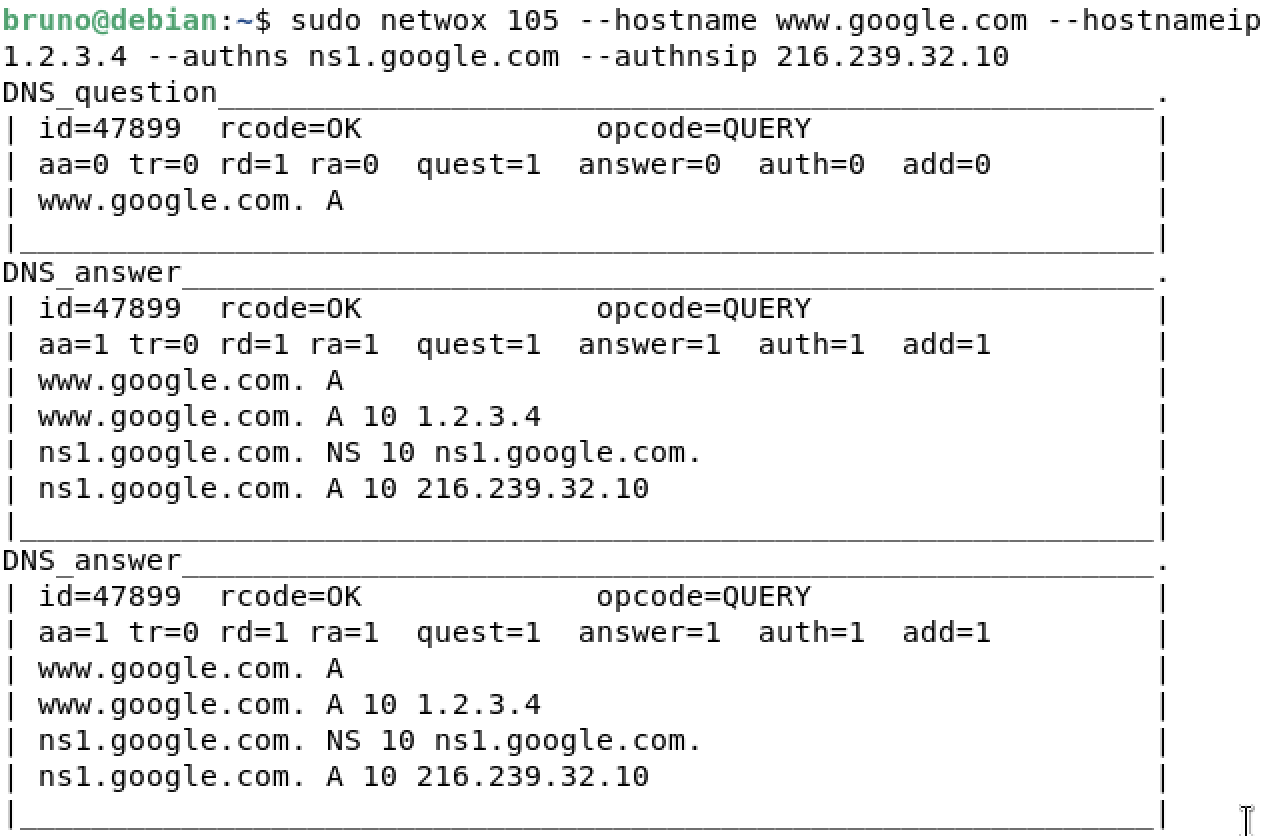
\includegraphics[scale=0.5]{images/netwox-google.png}
\end{center}

For task 6 and 7 we realize a DNS cache poisoning attack, this aims to make the effects of the spoofing attack almost permanent, this is done by changing the DNS server's cache to redirect the victim to the attacker's IP, the code bellow shows the changes made to the server's configuration file:

\begin{center}
  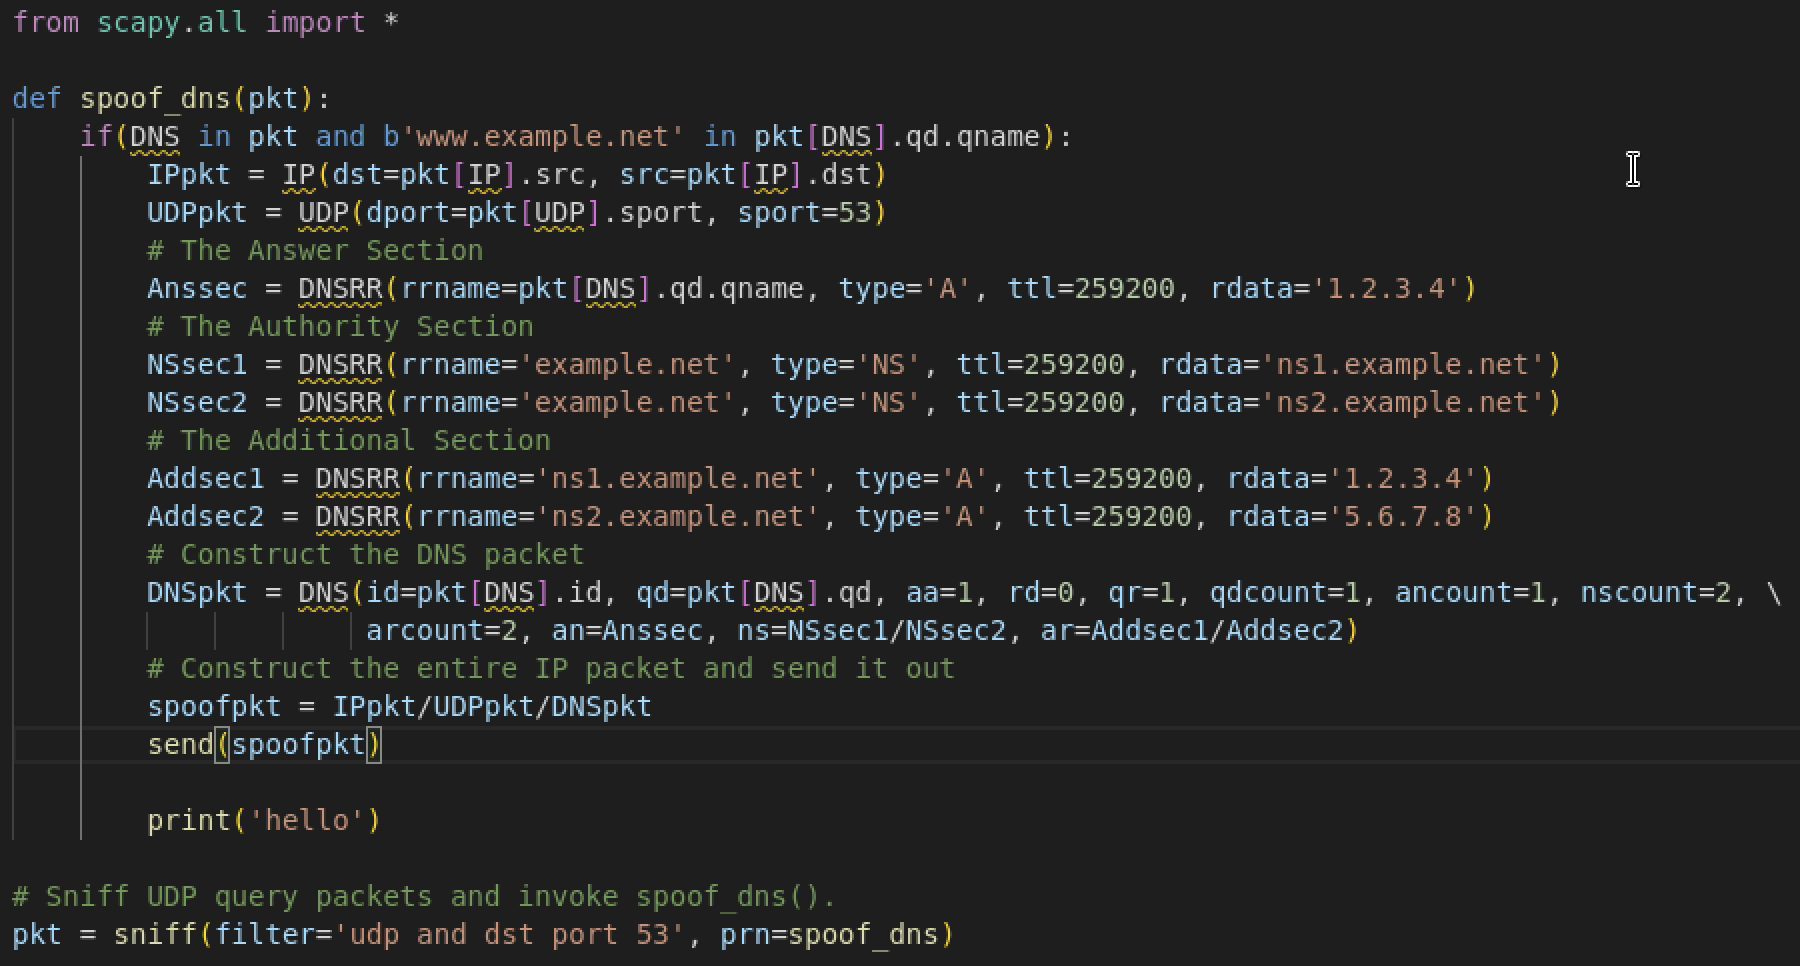
\includegraphics[scale=0.5]{images/Task7-code.png}
\end{center}

After running the code we can see that the server is now redirecting the victim to the attacker's IP, the result can be seen bellow:

\begin{center}
  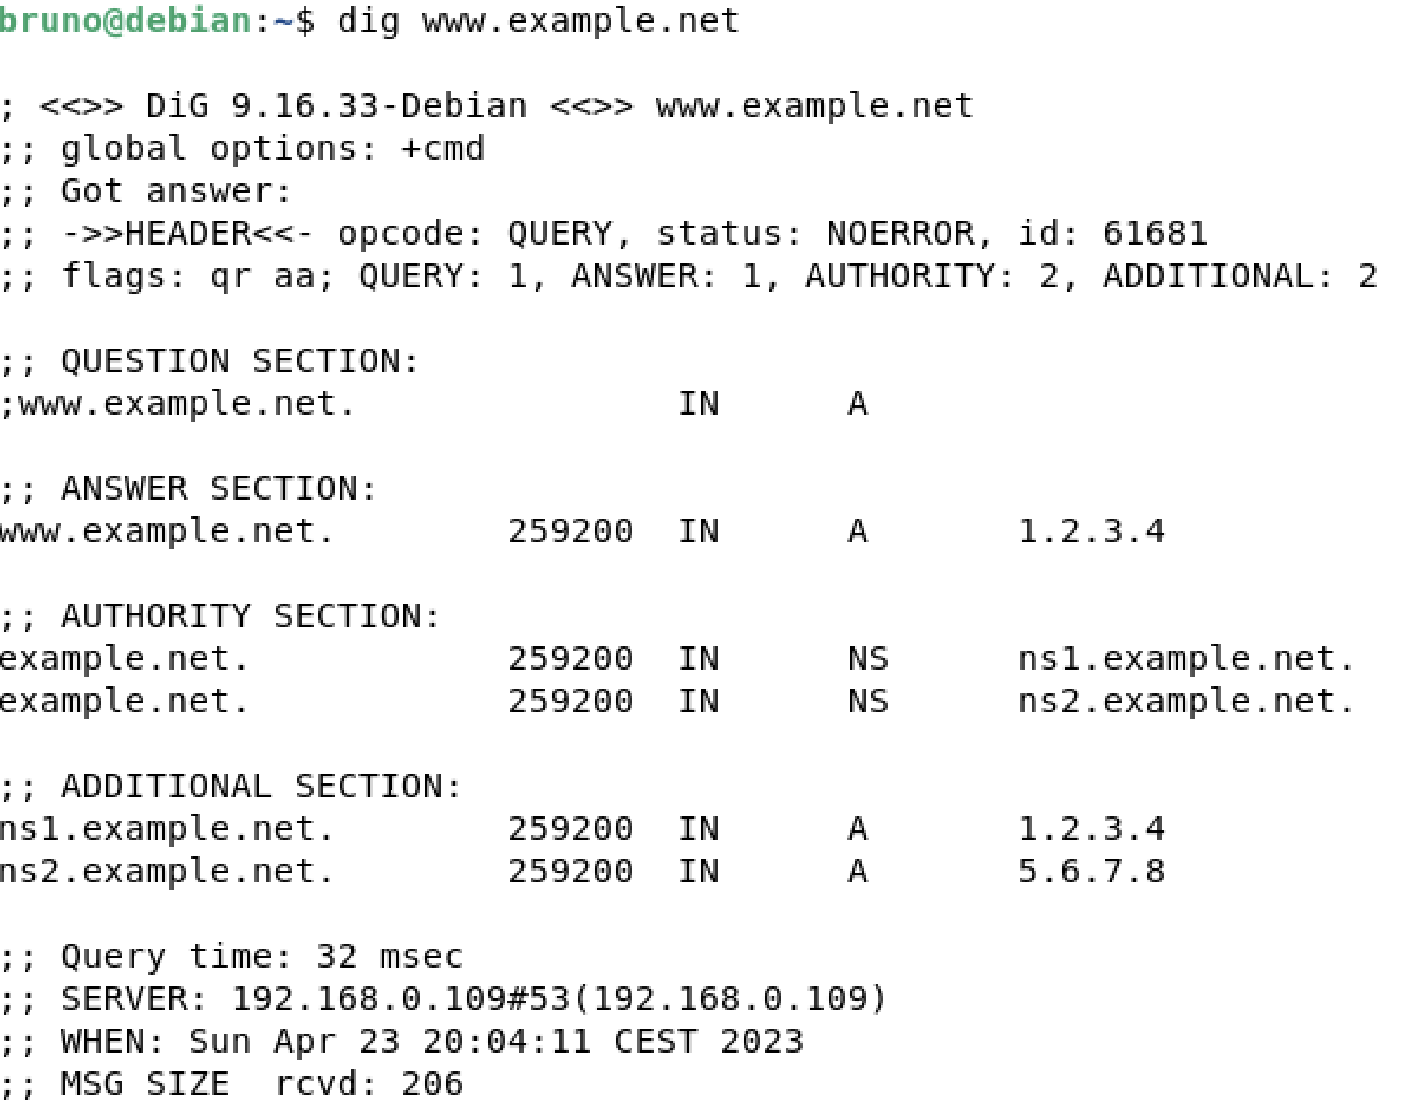
\includegraphics[scale=0.5]{images/Task7.png}
\end{center}

On task 8 we continue our attack but aiming another domain this time, for this we simply had to change the domain name on the code and run it again, the new code and result can be seen bellow:

\begin{center}
  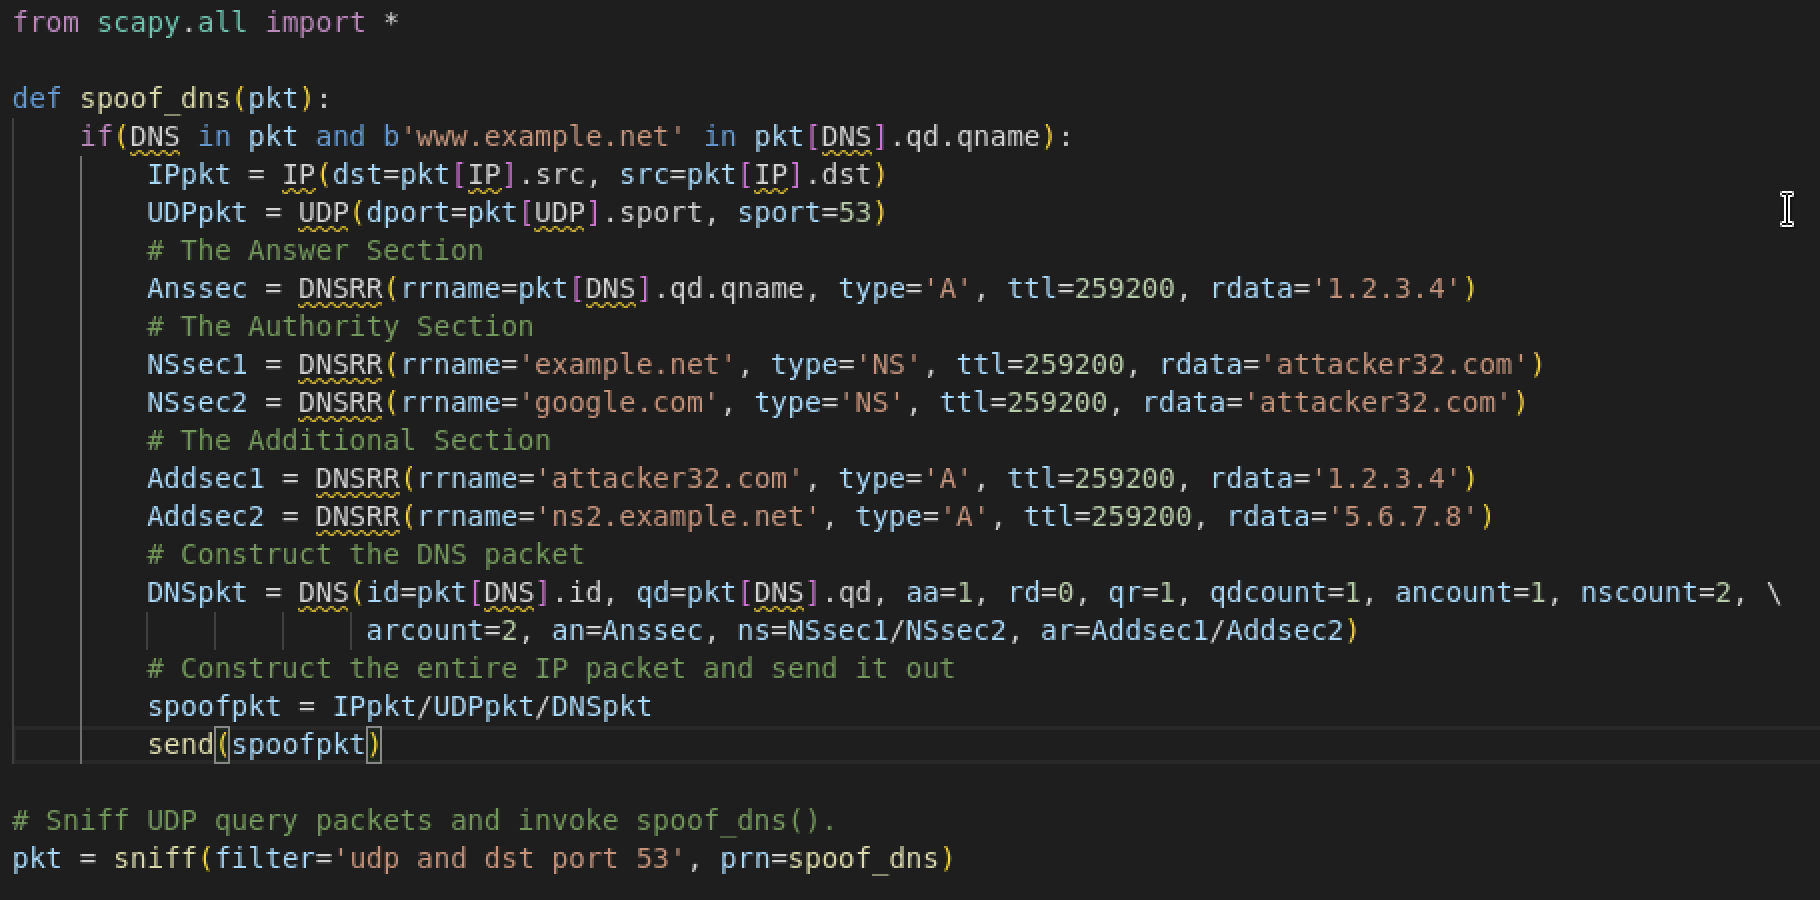
\includegraphics[scale=0.5]{images/Task8-code.png}
\end{center}

\begin{center}
  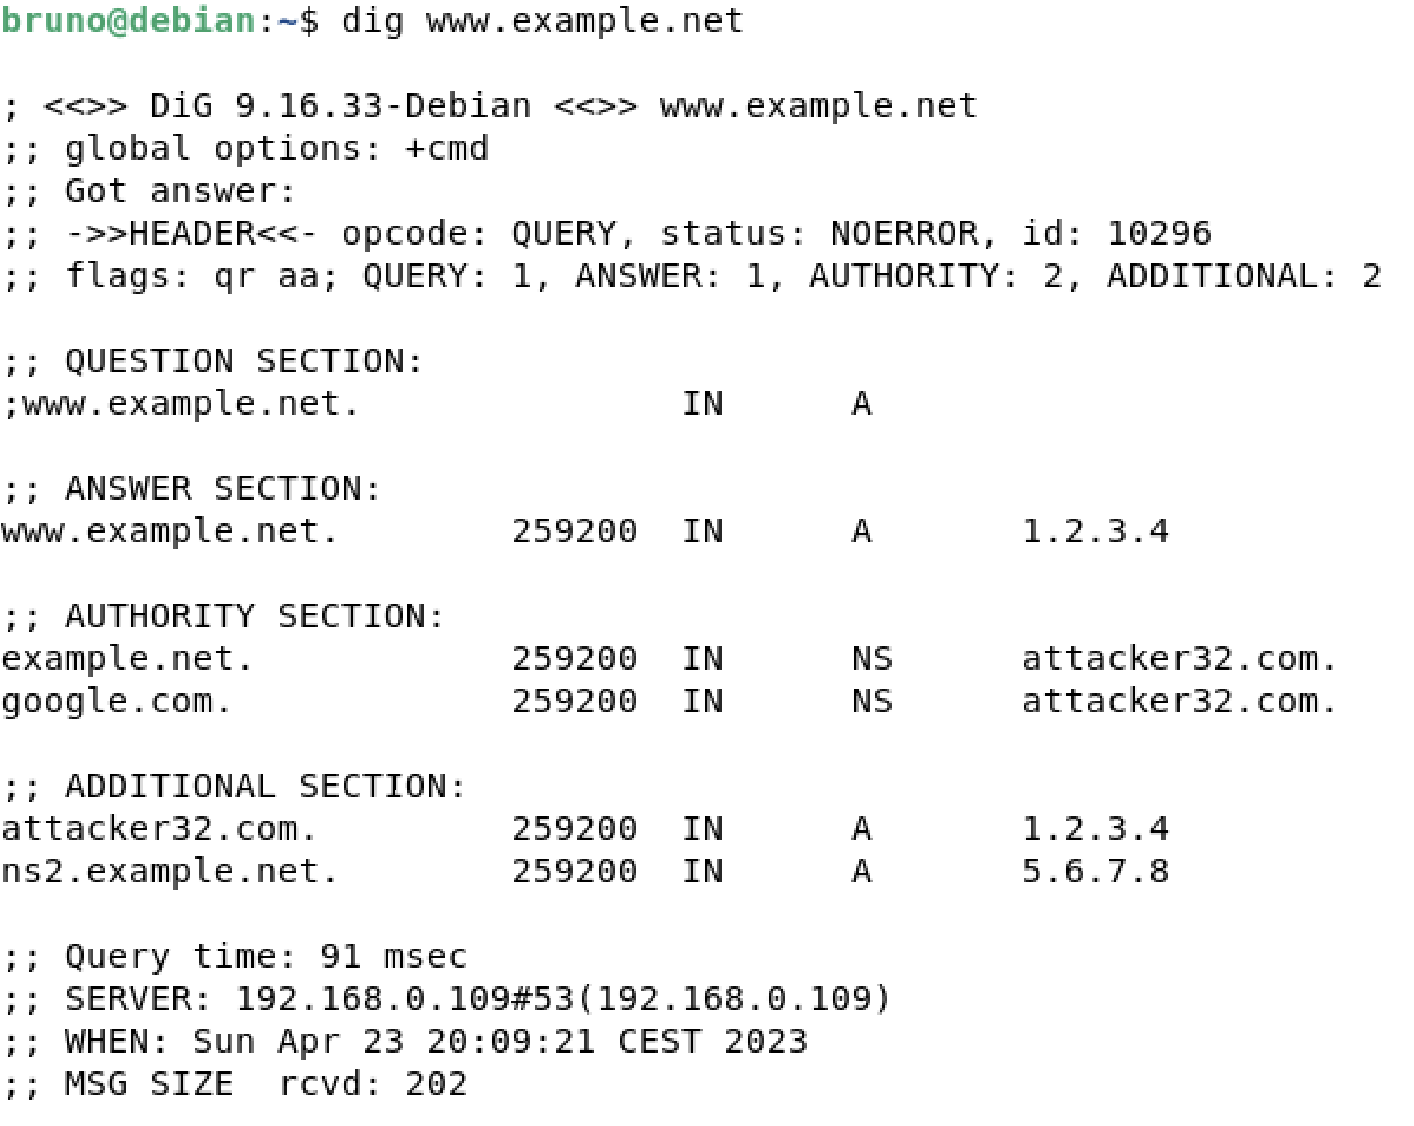
\includegraphics[scale=0.5]{images/Task8.png}
\end{center}

Finally for task 9 we target the additional information stored on a DNS request, for this we changed the authority and additional sections on the code which can be seen bellow:

\begin{center}
  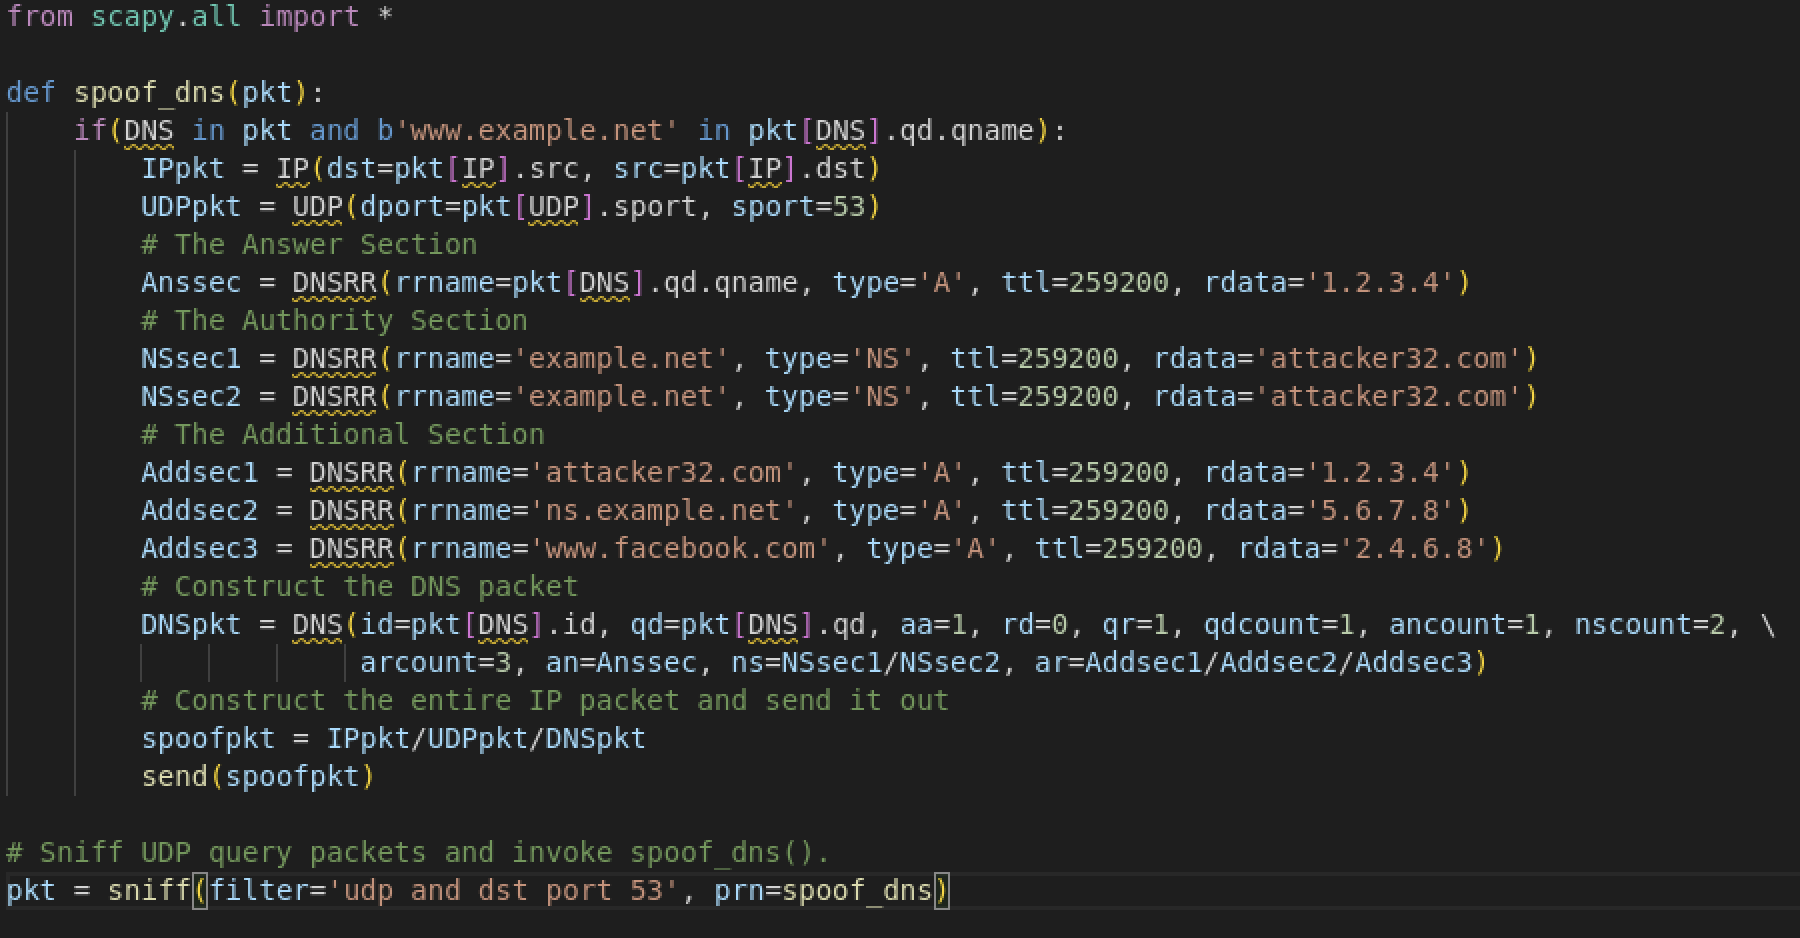
\includegraphics[scale=0.5]{images/Task9-code.png}
\end{center}

Running this new code we can see that the server is now redirecting the victim to the attacker's IP and also showing the additional information of the DNS, as seen in the figure:

\begin{center}
  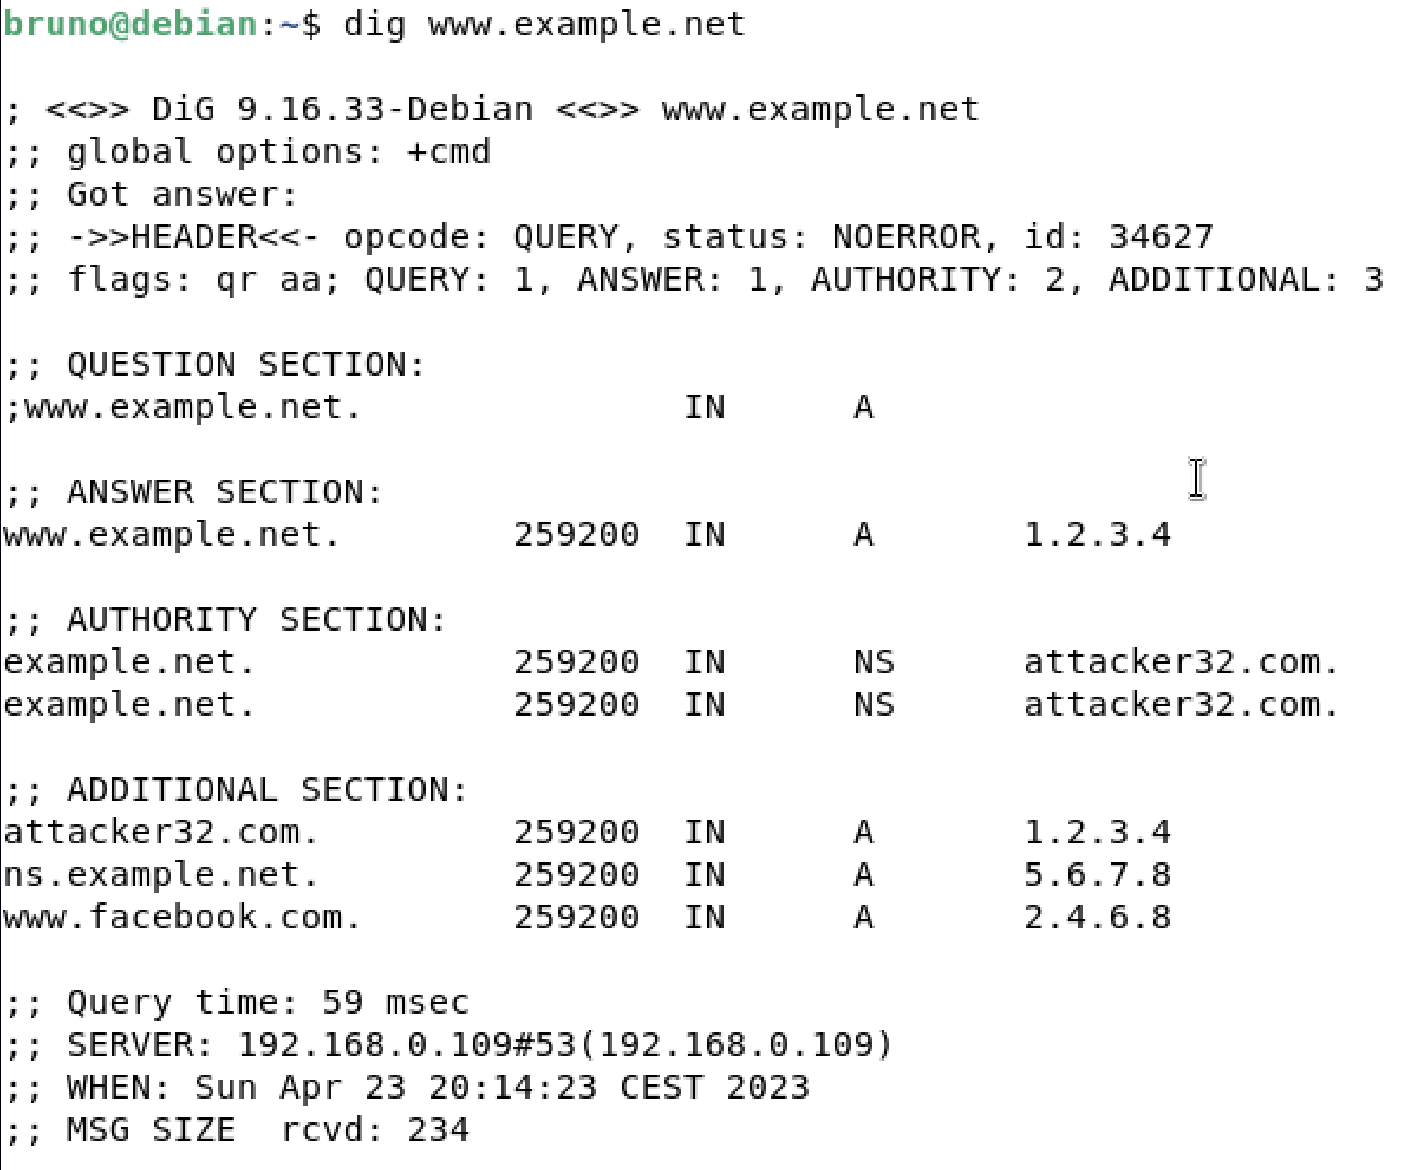
\includegraphics[scale=0.5]{images/Task9.png}
\end{center}

\pagebreak
\section{Conclusion}

This lab was essential on the understanding of the DNS server by allowing us to create and configure it first-hand.
We were able to fully understand how to configure, run and realize attacks on a DNS server, we also got more used to the Linux environment as it was necessary to configure files and run commands on the bash terminal.
On top of that we also gained knowledge on the form of communication between the machines by using the Wireshark and Scapy tool to visualize the traffic on the network and the packets sent.

\end{document}